% -----------------------------------------------------------------------------
%
% Copyright (c) 2017 Sam Cox, Roberto Sommariva
%
% This file is part of the AtChem2 software package.
%
% This file is covered by the MIT license which can be found in the file
% LICENSE.md at the top level of the AtChem2 distribution.
%
% -----------------------------------------------------------------------------

\chapter{Introduction} \label{ch:introduction}

\textbf{AtChem2} is an open source modelling tool for atmospheric
chemistry. It is designed to build and run zero-dimensional
box-models using the Master Chemical Mechanism
(\href{http://mcm.leeds.ac.uk/MCM/}{MCM}).  The \textbf{MCM} is a
near-explicit chemical mechanism which describes the gas-phase
oxidation of primary emitted Volatile Organic Compounds (VOC) to
carbon dioxide (\cf{CO2}) and water (\cf{H2O}). The MCM protocol is
detailed in \citet{jenkin_1997} and subsequent updates
\citep{saunders_2003, jenkin_2003, bloss_2005, jenkin_2015}. Although
it is meant to be used with the MCM, AtChem2 can use any other
chemical mechanism, as long as it is in the correct format
(Sect.~\ref{sec:chemical-mechanism}).

AtChem2 is a development of \textbf{AtChem-online}, a modelling web
tool created to facilitate the use of the MCM in the simulation of
laboratory and environmental chamber experiments within the
\href{https://www.eurochamp.org/}{EUROCHAMP} community
\citep{martin_2009}. AtChem-online runs as a web service -- provided
by the University of Leeds --and can be accessed at
\href{https://atchem.leeds.ac.uk/webapp/}{https://atchem.leeds.ac.uk/webapp/}:
in order to use AtChem-online, a user needs only a text editor, file
compression software, a web browser, and an internet connection. A
tutorial -- with examples and exercises -- is available on the MCM
\href{http://mcm.leeds.ac.uk/MCMv3.3.1/atchem/tutorial_intro.htt}{website}.

AtChem-online is easy to use even for inexperienced users but has a
number of limitations, mostly related to its nature as a web
application. AtChem2 was developed from AtChem-online with the
objective to provide an \emph{offline} modelling tool capable of
running long simulations of computationally intensive models, as well
as batch simulations for sensitivity studies. In addition, AtChem2
implements a continuous integration workflow, coupled with a
comprehensive suite of tests and version control software
(\href{https://git-scm.com/}{git}), which makes it robust, reliable
and traceable.

The codebase of AtChem2 is structured into four components (or layers)
-- as illustrated in Fig.~\ref{fig:atchem-arch} -- and is written
mostly in Fortran 90/95.  Installation, compilation and execution of
AtChem2 are semi-automated via a number of shell and Python scripts
that require minimal input from the user. This document
(\texttt{AtChem2-Manual.pdf}) is the AtChem2 user manual and contains
all the information required to install, set up and use the current
version of AtChem2. A summary of these instructions, and additional
information, can be found on the
\href{https://github.com/AtChem/AtChem2/wiki/}{wiki}.

\begin{figure}[htb]
  \centering
  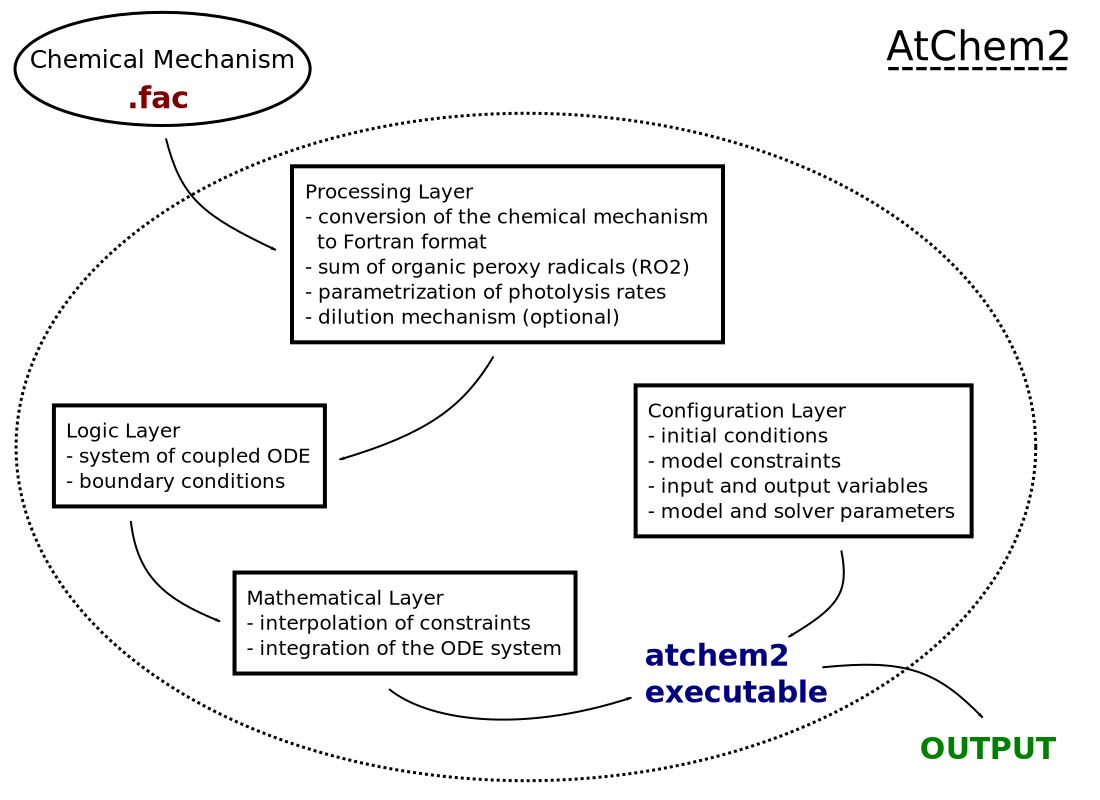
\includegraphics[width=0.8\textwidth]{atchem-structure.png}
  \caption{Architecture of AtChem2.}
  \label{fig:atchem-arch}
\end{figure}

% -------------------------------------------------------------------- %
\section{License and citation} \label{sec:license-citation}

AtChem2 is open source -- released under \textbf{MIT license} -- and is hosted
at \href{https://github.com/AtChem/AtChem2}{https://github.com/AtChem/AtChem2}.
A copy of the license can be found in the \texttt{LICENSE.md} file.

The model is free to use, compatible with the terms of the MIT
license; if used in a publication please include a citation to
the following paper:\\

R.~Sommariva, S.~Cox, C.~Martin, K.~Boro{\'n}ska, J.~Young, P.~K. Jimack,
M.~J. Pilling, V.~N. Matthaios, B.~S. Nelson, M.~J. Newland, M.~Panagi,
W.~J. Bloss, P.~S. Monks, and A.~R. Rickard.
\textbf{AtChem (version 1), an open-source box model for the Master Chemical Mechanism}.
\textit{Geoscientific Model Development}, 13, 1, 169--183, 2020.
doi: \href{https://doi.org/10.5194/gmd-13-169-2020}{10.5194/gmd-13-169-2020}.
